\documentclass[11pt,a4paper]{article}
\usepackage[margin=21mm]{geometry}
\usepackage{amsmath,amssymb,booktabs,array,tikz,enumitem,hyperref}
\usetikzlibrary{arrows.meta,positioning}
\setlength{\parindent}{0pt}\setlength{\parskip}{6pt}
\newcommand{\question}[2]{\section*{#1}}
\newcommand{\board}[1]{\begin{tikzpicture}[x=0.39cm,y=0.39cm,baseline={([yshift=-.5ex]current bounding box.center)}]
\draw(0,0)rectangle(3,3);\foreach\i in{1,2}{\draw(\i,0)--(\i,3);\draw(0,\i)--(3,\i);}
\foreach[count=\i from 0]\v in{#1}{\pgfmathtruncatemacro{\c}{mod(\i,3)}\pgfmathtruncatemacro{\r}{floor(\i/3)}\node at(\c+0.5,2.5-\r){\v};}
\end{tikzpicture}}
\newcommand{\blank}{}
\tikzset{box/.style={draw,rounded corners,align=center,inner sep=6pt},arr/.style={->,>=Stealth}}
\begin{document}
\begin{center}{\Large\bfseries Homework 3: Concise Answers}\\[4pt]Formulae, tables, and diagrams\end{center}

\question{Games1 (p.\ 1)}{Chinese chess branching factor}
\textbf{(A)} $x=1,\ldots,9$: left to right; $y=0,\ldots,9$: bottom to top. Red moves toward increasing $y$.
\begin{center}\small\begin{tabular}{l|c|p{7.9cm}|r}\toprule
Piece&Position&Legal destination(s) / directional count&Count\\\midrule
Left rook&$(1,0)$&$(1,1),(1,2),(1,3)$&3\\
Right rook&$(9,0)$&$(9,1),(9,2)$&2\\
Left horse&$(2,0)$&$(1,2),(3,2)$&2\\
Right horse&$(8,0)$&$(7,2),(9,2)$&2\\
Left elephant&$(3,0)$&$(1,2),(5,2)$&2\\
Right elephant&$(7,0)$&$(5,2),(9,2)$&2\\
Left advisor&$(4,0)$&$(5,1)$&1\\
Right advisor&$(6,0)$&$(5,1)$&1\\
General&$(5,0)$&$(5,1)$&1\\
Left cannon&$(4,2)$&Left 3, right 3, down 1, up 6&13\\
Right cannon&$(8,2)$&Left 3, right 1, down 1, up 4 noncaptures + 1 capture&10\\
Soldier 1&$(1,4)$&$(1,5)$&1\\
Soldier 2&$(3,3)$&$(3,4)$&1\\
Soldier 3&$(5,3)$&$(5,4)$&1\\
Soldier 4&$(7,3)$&$(7,4)$&1\\
Soldier 5&$(9,3)$&$(9,4)$&1\\\bottomrule\end{tabular}\normalsize\end{center}
Right cannon capture: $(8,2)\to(8,9)$, with the single screen at $(8,7)$.


\[
b=3+2+2+2+2+2+1+1+1+13+10+5=\boxed{44}.
\]


\textbf{(B)} One-ply leaf evaluations:
\[\boxed{44\text{ heuristic evaluations}}.\]
\textbf{(C)} Three-ply leaf evaluations (constant $b$):
\[\boxed{b^3=44^3=85,184\text{ heuristic evaluations}}.\]
If every non-root node is evaluated: $44+44^2+44^3=87,164$.

\newpage
\question{Game2 (p.\ 2)}{Finish the two incomplete games}
Cell numbering:
\begin{center}\board{1,2,3,4,5,6,7,8,9}\end{center}
$X$ first; alternating moves. Two legal continuations:

\textbf{First game.} The supplied prefix is $X2,O5,X3,O1$. Add
\[\boxed{X9,\ O6,\ X4,\ O7,\ X8}.\]
\begin{center}
\board{O,X,X,\blank,O,\blank,\blank,\blank,\blank}$\;\to\;$
\board{O,X,X,\blank,O,\blank,\blank,\blank,X}$\;\to\;$
\board{O,X,X,\blank,O,O,\blank,\blank,X}\\[9pt]
\board{O,X,X,X,O,O,\blank,\blank,X}$\;\to\;$
\board{O,X,X,X,O,O,O,\blank,X}$\;\to\;$
\board{O,X,X,X,O,O,O,X,X}
\end{center}
$\boxed{\text{Draw}}$ (no winning line).

\textbf{Second game.} The supplied prefix is $X2,O3$. Add
\[\boxed{X5,\ O8,\ X1,\ O9,\ X6,\ O4,\ X7}.\]
\begin{center}
\board{\blank,X,O,\blank,\blank,\blank,\blank,\blank,\blank}$\;\to\;$
\board{\blank,X,O,\blank,X,\blank,\blank,\blank,\blank}$\;\to\;$
\board{\blank,X,O,\blank,X,\blank,\blank,O,\blank}$\;\to\;$
\board{X,X,O,\blank,X,\blank,\blank,O,\blank}\\[9pt]
\board{X,X,O,\blank,X,\blank,\blank,O,O}$\;\to\;$
\board{X,X,O,\blank,X,X,\blank,O,O}$\;\to\;$
\board{X,X,O,O,X,X,\blank,O,O}$\;\to\;$
\board{X,X,O,O,X,X,X,O,O}
\end{center}
$\boxed{\text{Draw}}$ (no winning line).

\newpage
\question{Game3 (p.\ 3)}{Bottom-up value backup}
$U=+1$ ($X$ win), $-1$ ($O$ win), $0$ (draw).
\[
V(s)=\begin{cases}U(s),&s\text{ terminal},\\
\max_{s'\in\mathrm{children}(s)}V(s'),&X\text{ to move},\\
\min_{s'\in\mathrm{children}(s)}V(s'),&O\text{ to move}.
\end{cases}
\]
Terminal values:
\begin{center}
\board{X,O,X,\blank,O,X,O,\blank,X}\quad$+1$\qquad
\board{X,\blank,X,O,O,X,O,\blank,X}\quad$+1$.
\end{center}
Upper fork:
\begin{center}
\board{X,X,O,O,O,X,X,O,X}\quad$0$\qquad
\board{X,O,O,O,O,X,X,X,X}\quad$+1$.
\end{center}
Upper fork: $\min(0,1)=0$; parent $\min(1,0)=0$. Single-successor chains retain the value.

Shared fork:
\begin{center}
\board{O,X,X,X,X,O,O,O,X}\quad$0$\qquad
\board{O,X,X,X,X,O,O,X,O}\quad$+1$.
\end{center}
Shared fork: $\min(0,1)=0$.

First $X$: corner. Pictured $O$ replies:
\[
O\text{ in center}:0,\qquad O\text{ in top-right corner}:1,
\qquad O\text{ on top edge}:1.
\]
Dashed draw alternative at an $X$ node: $\max(1,0)=1$.

Opening backup:
\[
V(\text{corner first})=\min(0,1,1)=0,\quad
V(\text{center first})=\min(0,1)=0,
\quad V(\text{root})=\max(0,0)=\boxed{0}.
\]


Opening tree (single-successor chains compressed):
\begin{center}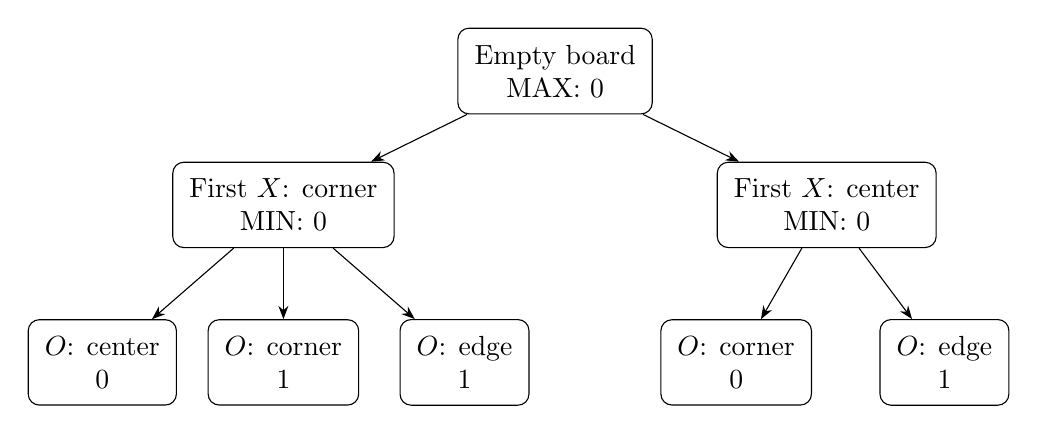
\begin{tikzpicture}[x=1.15cm,y=1cm]
\node[box](root)at(0,0){Empty board\\MAX: $0$};
\node[box](corner)at(-3,-1.7){First $X$: corner\\MIN: $0$};
\node[box](center)at(3,-1.7){First $X$: center\\MIN: $0$};
\node[box](c1)at(-5,-3.7){$O$: center\\$0$};
\node[box](c2)at(-3,-3.7){$O$: corner\\$1$};
\node[box](c3)at(-1,-3.7){$O$: edge\\$1$};
\node[box](m1)at(2,-3.7){$O$: corner\\$0$};
\node[box](m2)at(4.3,-3.7){$O$: edge\\$1$};
\foreach\a/\b in{root/corner,root/center,corner/c1,corner/c2,corner/c3,center/m1,center/m2}\draw[arr](\a)--(\b);
\end{tikzpicture}\end{center}
$\boxed{\text{Choose center}}$; corner ties at value $0$.

Values apply to the supplied partial graph. In the full game, perfect play draws from every opening.

\newpage
\question{Game4 (p.\ 4)}{Two-step look-ahead with a heuristic}
Initial board:
\begin{center}\board{\blank,O,\blank,\blank,X,\blank,\blank,\blank,\blank}\end{center}
$h(s)=\#\text{open }X\text{ lines}-\#\text{open }O\text{ lines}$. MIN over $O$ replies:
\begin{center}\begin{tabular}{l|l|c}\toprule
$X$'s candidate move&Scores after $O$'s responses&MIN value\\\midrule
Top-left corner&$2,1,3,1,2,1$&1\\
Middle-left edge&$1,0,2,0,1,1$&0\\
Bottom-left corner&$2,2,3,1,2,2$&1\\
Bottom-middle edge&$1,1,0$ (symmetry representatives)&0\\\bottomrule\end{tabular}\end{center}
Root backup:
\[\max(1,0,1,0)=\boxed{1}.\]
$\boxed{\text{Best: all four corners (by symmetry)}}$.

Choose bottom-left as a tie-break: same worst-case value $1$, more favorable other reply scores.

\begin{center}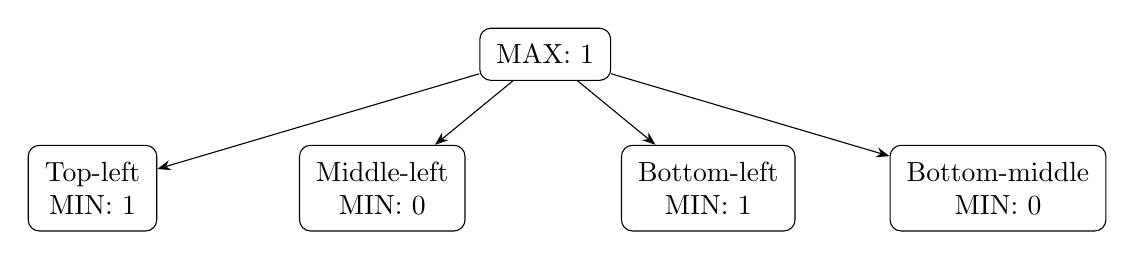
\begin{tikzpicture}[x=1.15cm,y=1cm]
\node[box](root)at(0,0){MAX: $1$};
\node[box](a)at(-5,-1.7){Top-left\\MIN: $1$};\node[box](b)at(-1.8,-1.7){Middle-left\\MIN: $0$};
\node[box](c)at(1.8,-1.7){Bottom-left\\MIN: $1$};\node[box](d)at(5,-1.7){Bottom-middle\\MIN: $0$};
\foreach\n in{a,b,c,d}\draw[arr](root)--(\n);
\end{tikzpicture}\end{center}
Chosen move:
\begin{center}\board{\blank,O,\blank,\blank,X,\blank,X,\blank,\blank}\end{center}

\newpage
\question{Game5 (pp.\ 5--6)}{Properties of the complete search tree}
$X$ first; root depth $0$; stop immediately after a win or a full board.
Leaves count move histories (no board or symmetry merging).

\begin{center}\begin{tabular}{c|l|c}\toprule
Item&Reason&Result\\\midrule
1&Third $X$ mark: move 5; full board: move 9&Leaf depths $5,6,7,8,9$\\
2&Depth 5: $X$ has 3 marks, $O$ has 2&$U_5=+1$\\
3&Move 6 is $O$'s; earlier $X$ wins already stopped&$U_6=-1$\\
4&Move 9 is $X$'s: win or full-board draw&$U_9\in\{0,+1\}$\\\bottomrule
\end{tabular}\end{center}

\textbf{5. Number of depth-5 leaves.}
$8$ winning lines; $3!$ orders for $X$; $\binom62 2!$ placements/orders for $O$.
\[
N_5=8\times3!\times\binom62\times2!
=8\times6\times15\times2=\boxed{1,440}.
\]

\textbf{6. Number of depth-6 leaves (optional).}
Count $O$ wins, then exclude earlier $X$ wins:
\[
8\times3!\times\binom63\times3!=5,760.
\]
Disjoint ordered winning-line pairs: $3\cdot2+3\cdot2=12$. Invalid orders per pair: $3!3!=36$.
\[
N_6=5,760-12\times36=\boxed{5,328}.
\]


\textbf{7. Depth-9 leaves (optional).} $L_d(s,t)$ counts terminal continuations in exactly $d$ further moves:
\[
L_0(s,t)=\begin{cases}1,&s\text{ is terminal},\\0,&\text{otherwise},\end{cases}
\]
and for $d>0$,
\[
L_d(s,t)=\begin{cases}
0,&s\text{ is terminal},\\
\displaystyle\sum_{a\in\mathrm{legal}(s,t)}L_{d-1}(\mathrm{Result}(s,a),\bar t),&\text{otherwise}.
\end{cases}
\]
Enumeration of the unmerged legal tree:
\begin{center}\begin{tabular}{c|r|r|r|r}\toprule
Depth&$X$ wins&$O$ wins&Draws&Terminal histories\\\midrule
5&1,440&0&0&1,440\\
6&0&5,328&0&5,328\\
7&47,952&0&0&47,952\\
8&0&72,576&0&72,576\\
9&81,792&0&46,080&127,872\\\bottomrule\end{tabular}\end{center}
Thus
\[
\boxed{N_9=81,792+46,080=127,872}.
\]
Check: $16$ full draw boards; every mark order is legal:
\[
16\times5!\times4!=46,080.
\]
Total terminal histories:
\[
1,440+5,328+47,952+72,576+127,872=255,168.
\]
$9!$ is invalid: it includes histories continuing after an earlier win.
\end{document}
